
%(BEGIN_QUESTION)
% Copyright 2015, Tony R. Kuphaldt, released under the Creative Commons Attribution License (v 1.0)
% This means you may do almost anything with this work of mine, so long as you give me proper credit

Read and outline the ``Fiber Optic Data Communication'',  ``Fiber Optic Cable Construction'', ``Fiber Optic Cable Connectors, Routing, and Safety'', and ``Fiber Optic Cable Testing'' sections of the ``Instrument Connections'' chapter in your {\it Lessons In Industrial Instrumentation} textbook.  Note the page numbers where important illustrations, photographs, equations, tables, and other relevant details are found.  Prepare to thoughtfully discuss with your instructor and classmates the concepts and examples explored in this reading.

\underbar{file i02744}
%(END_QUESTION)





%(BEGIN_ANSWER)


%(END_ANSWER)





%(BEGIN_NOTES)

Optical fiber acts as a ``pipe'' to convey light between two points.  If digital communication equipment is equipped with LED sources and photodetectors, optical fibers may replace copper-wire cabling between the equipment as a data-communication pathway.  This equipment commonly has two fiber ports, one for {\it transmit} and one for {\it receive}.

\vskip 10pt

``ST'' style fiber connectors act like miniature BNC connectors, with quarter-turn locking rings to hold them in place.  Older ``SMA'' connectors used threaded barrels.  ``SC'' connectors designed for fiber {\it pairs}.

\vskip 10pt

Advantages of optical fiber over copper wire:

\begin{itemize}
\item{} Much greater bandwidth (measured in terahertz!)
\item{} Much less signal loss
\item{} Immunity from noise
\item{} No radiation loss from cable -- can't eavesdrop
\item{} Safe to route near high voltage (doesn't conduct)
\item{} Galvanic isolation (doesn't conduct)
\item{} Safe in explosive environments
\end{itemize}

\vskip 10pt

Disadvantages of optical fiber compared to copper wire:

\begin{itemize}
\item{} Requires large bend radii
\item{} Connections must be very clean
\item{} Special tools required for installation and maintenance
\item{} Special tools required for testing
\end{itemize}

\vskip 10pt

Optical fiber made from fused silica, a core surrounded by a cladding.  The core and cladding have differing indices of refraction necessary to ``channel'' light and keep it within the cable by means of {\it total internal reflection}.

\vskip 10pt

Snell's Law states that the sine values of incident and refracted light ray angles at an interface between two different materials is proportional to the speed of light in each material:

$${{\sin \theta_1} \over v_1} = {{\sin \theta_2} \over v_2}$$

If the incident light ray angle within the slower-light material reaches or exceeds a certain value, the light internally reflects off the interface and never enters the faster-light material.  This is what we do with optical fiber: the core has a slower speed of light than the cladding, therefore so long as the light enters the core at a shallow enough angle relative to the centerline, it reflects off the cladding and never leaves the core.

\vskip 10pt

Core and cladding diameters measured in {\it microns} (millionths of a meter).  62.5/125 common in the US, 50/125 common in Europe.  Other sizes available too.  Plastic jacketing (typically 250 microns diameter) layered on top forms a Primary Coated Optical Fiber (PCOF).  More plastic jacketing (typically 900 microns diameter) and additional materials such as Kevlar or fiberglass strength fibers added to make Secondary Coated Optical Fiber (SCOF) suitable for end-use.  Large cables often wrap several PCOF within a tough sheath.

\vskip 10pt

Fiber termination can be painstaking work: stripping the fiber down to core and cladding, cleaving the fiber flat, and securing to a connector using epoxy or hot-melt adhesive.  Finally, the fiber end must be polished to a flat, smooth surface.  Splicing may be done with ``butt'' connectors (some filled with an optical gel matching the refractive index of the fiber) or may be done by melting the two glass fibers together ({\it fusion} splicing).

\vskip 10pt

If an optical fiber is bent too sharply, the critical angle for total internal reflection may be exceeded, causing light to leak out of the fiber.  For this reason, there is a minimum bend radius for fiber installation.  A cable tie attached too tightly to an optical fiber will kink the fiber and cause this kind of loss.

\vskip 10pt

Optical fibers pose a safety hazard when terminating: the slivers of glass may embed in your skin and are nearly impossible to extract because they're do hard to see.  Powered fibers pose a vision hazard by the intensity of the light emitted.  This is especially true where laser light sources are used.  Keep in mind that some optical systems use infra-red light which can't be seen at all!  Some data communication equipment is equipped with Open Fiber Control (OFC) which is a feature shutting off all light if ever a fiber becomes unplugged.

\vskip 10pt

Optical fibers may be tested by measuring light lost from end to end (using an optical source and power meter), or by shooting a brief pulse of light down the fiber and analyzing the back-scattered light (using an Optical Time-Domain Reflectometer, or OTDR).  End-to-end power tests may reveal a number of problems, but not pinpoint {\it which} type of problem is responsible for the loss, or {\it where} that problem is located.  OTDR testing can pinpoint both the type of loss and its location.  Optical cable flaws include:

\begin{itemize}
\item{} Poor fiber alignment within connectors
\item{} Mismatched fiber sizes
\item{} Dirty connector ends
\item{} Improperly polished fiber ends
\item{} Minimum bend radius violated
\item{} Cracked fiber core
\end{itemize}

OTDR testing works on the principle of the incident light pulse losing photons due to scattering in the glass.  This scattering sends a continuous ``echo'' back toward the light source as the light packet travels along the fiber's length.  Reflective discontinuities result in an upward jump on the OTDR trace, while non-reflective discontinuities result in a downward jump on the OTDR trace.  The flaw's location is revealed by the horizontal distance between the incident pulse and the flaw, as shown on the time-domain trace.  Beware the difference between fiber length and cable length, as individual PCOF fibers may spiral along the length of a larger cable!



\vskip 20pt \vbox{\hrule \hbox{\strut \vrule{} {\bf Suggestions for Socratic discussion} \vrule} \hrule}

\begin{itemize}
\item{} Explain how light is constrained within an optical fiber.
\item{} Identify advantages enjoyed by optical fiber over copper cable.
\item{} Identify advantages enjoyed by copper cable over optical fiber.
\item{} Explain how Snell's Law relates to optical fiber operation.
\item{} Explain why optical fibers must have a minimum bend radius.
\item{} Describe how optical fibers may be spliced together to form a longer fiber.
\item{} Identify some unique safety hazards when working with optical fiber.
\item{} Explain how some of the common fiber testing methods work.
\end{itemize}









\vfil \eject

\noindent
{\bf Prep Quiz:}

Identify {\it two} distinct advantages fiber-optic cables enjoy over copper cables for the purpose of signal communication.












\vfil \eject

\noindent
{\bf Summary Quiz:}

Contrast event \#3 versus event \#4 on this OTDR trace, providing an explanation for what might cause each one and why their shapes differ:

$$\includegraphics[width=15.5cm]{i02744x01.eps}$$










%INDEX% Reading assignment: Fiber optics

%(END_NOTES)

